\documentclass[10pt, a4paper]{article}
\usepackage[slovene]{babel}
\usepackage[utf8]{inputenc} %za šumnike
\usepackage{lmodern}
\usepackage[T1]{fontenc}
\usepackage{eurosym}

%slike:
\usepackage{graphicx}
\graphicspath{ {./slike/} }

\begin{document}

\begin{center}
\Huge \textbf{Naslov Skupina 19: Graffiti conjecture 232} \\
\medskip
\Large Urban Merhar, Martin Kokošinek\\
\end{center}

\section{Navodilo}
Računalniško generirana domneva trdi: Če je $G$ enostaven povezan graf, potem
\begin{center}
 $2\gamma_{t}(G) \geq rad(G) + ecc(B)$.
\end{center}
 
Preveri domnevo na različne načine za male in velike grafe. Z uporabo populacijske metahevristike, preveri domnevo v upanju, da jo ovržeš.

\medskip
Nekaj pripomb:

\begin{enumerate}
\item $ecc(v)$ je $ekscentričnost$ od vozlišča $v$. Ekscentričnost od $v$ je razdalja do najbolj oddaljenega vozlišča od vozlišča $v$, i.e., $ max\{d(v,u): u$ je vozlišče na grafu $\}$.
\item $rad(G)$ je $radij$ grafa, t.j., minimum vseh ekscentričnosti vozlišč grafa $G$.
\item $B$ je $obrobje$ grafa $G$, t.j., množica vozlišč z maksimalno ekscentričnostjo.
\item $ecc(S)$ je $ekscentričnost$ množice vozlišč $S$. Definirana je kot: Naj bo $S$ podmnožica množice vozlišč $V$. Razdalja med vozliščem $v$ in množico $S$, definirajmo kot razdaljo od $v$ do najbližjega volišča v $S$. $ecc(S)$ je maksimum razadalj od vozlišča v $V\backslash S$ do množice $S$.
\end{enumerate}


\section{Kratek opis}
$Computer\ generated\ conjectures$ so računalniško ustvarjene domneve. $Graffiti$ je računalniški program, ki generira te matematične domneve oziroma odprte probleme. Računalniši program $Graffiti$ je ustvaril $Siemion\ Fajtlowicz$.\\

V najinem projektu pri predmetu Finančni praktikum si bova ogledala $Graffiti$ $conjecture$ $232$, ki jo bova testirala za majhne in velike grafe v upanju, da najdeva protiprimer. Ideja je, da enačbo zapiševa v programskem jeziku $Sage$ in generirava naključne grafe. Na vsakem od teh grafov pa predpostavko testirava.\\


Že vgrajene funkcije, ki jih bova uporabila v programu:
\begin{enumerate}
	\item $dominating\_ set(total=True, value\_ only=True)$ vrne najmanjšo dominirajočo množico na grafu $G$.
	\item $radius()$ vrne radij grafa $G$.
	\item $eccentricity()$ vrne ekscentričnost vozlišča $v$.
	\item $periphery()$ vrne množico vozlišč iz obrobja grafa $G$.
\end{enumerate}

\subsection{Razlaga pojmov}
\begin{itemize}
\item Dominirajoča Množica $D$: $D$ je množica, kjer je vsako vozlišče iz $G \backslash D$ sosed nekega vozlišča iz $D$.
\item Totalno Dominirajoča množica (TDM): Dominirajoči množici $D$ dodamo pogoj, da so tudi vozlišča dominirajoče množice 
$D$ sosedi vozlišč iz $D$.
\item Totalno Dominirajoče Število (TDŠ): Moč totalno dominirajoče množice grafa $G$.
\item $\gamma_{t}(G)$ je TDŠ grafa $G$.
\end{itemize}

\subsubsection{Populacijska metahevristika}
\textbf{Hevristika} (iz Grščine: 'najdem, odkrijem'): V računalništvu in matematični optimizaciji je visoko-nivojski način reševanja problemov, ko so klasični postopki prepočasni oziroma, ko klasične metode ne vrnejo točnih rezultatov. V zameno za polnost, optimalnost, natančnost, raje pridobimo na časovni zahtevnosti. \\
\textbf{Meta-hevristika} (meta iz Grščine: 'za, onstran') oziroma v prevodu Izčrpna-hevristika: Metahevristika vzame množico rešitev, ki je prevelika za analizo in s pomočjo določenih predpostavk glede optimizacije vrne zadovoljivo rešitev. Ta ni nujno globalno optimalna. \\
\textbf{Populacijska metahevristika}: Ohranjamo večje število kandidatov za rešitev in jih izboljšujemo s pomočjo populacijsih karakteristik. Primer je particle swarm optimization (PSO).

\section{Plan dela}
Zapisati učinkovit algoritem, ki bo za vsak generiran graf preverila lastnosti grafa in posledično domnevo. Za grafe, kjer  domneva ne bi držala pa nam izpiše graf in vrne vrednosti lastnosti, ki so potrebovane v domnevi.

\section{Potek dela}

Razlaga programa...

\section{Majhni grafi}

Majhne grafe sva v $sagu$ generirala s pomočjo funkcije $graphs.nauty\_geng('v\ -c')$. Kjer je $v$ število vozlišč grafa, $-c$ pa pomeni, da so grafi povezani. Na dovolj majhnih grafih sva generirala vse možne enostavne in povezane grafe ter na njih testirala predpostavko. Prav vsi grafi so ji ustrezali, zato sva se odločila podrobneje pogledati grafe, kjer je bila razlika med levo in desno stranjo predpostavke najmanjša.

Graf na dveh vozliščih. Razlika v predpostavki je $0$.

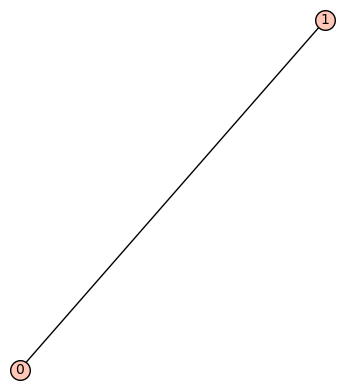
\includegraphics[width=5cm]{min_graf_2}

Graf na treh vozliščih. Razlika je $0$.

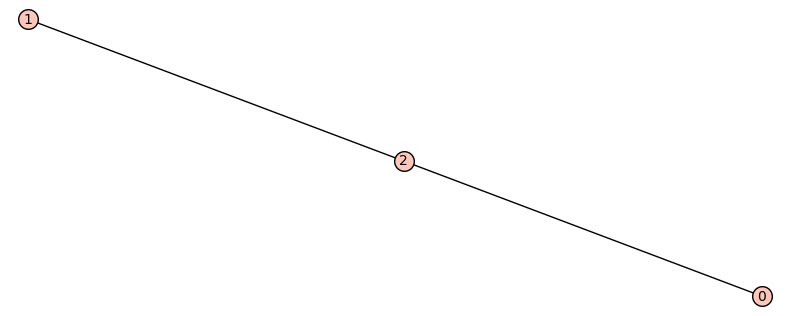
\includegraphics[width=5cm]{min_graf_3}

Grafi na štirih vozliščih imajo ponovno razliko predpostavke enako $0$. Izmed $6$ generiranih grafov imamo $2$ z razliko predpostavke $0$.

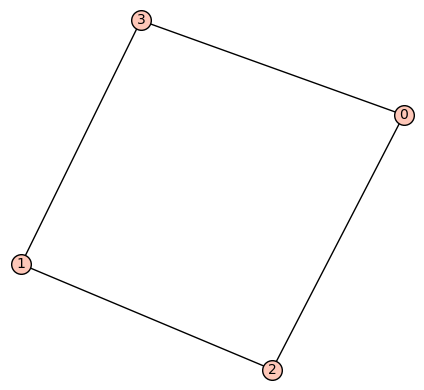
\includegraphics[width=5cm]{min_graf_4.1}
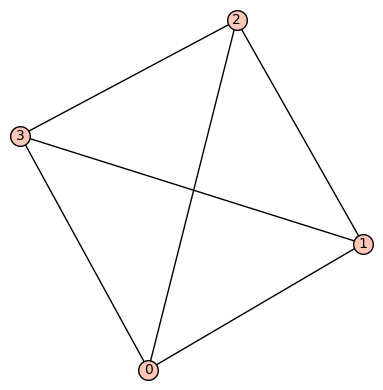
\includegraphics[width=5cm]{min_graf_4.2}

Pri grafih generiranih na petih vozliščih dobiš več grafov katerih razlika predpostavke je $0$. Generiranih je skupno $21$ grafov na pet vozliščih, od katerih jih $5$ ime razliko predpostavke $0$. Program testira vse te grafe v manj kot $0.07$ sekunde.

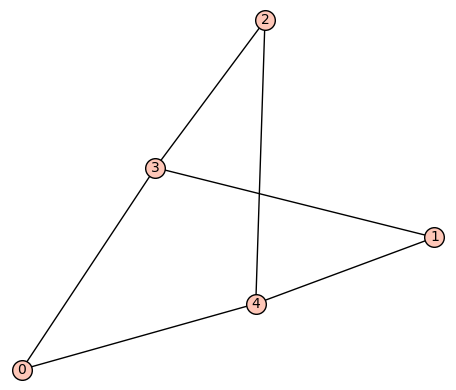
\includegraphics[width=5cm]{min_graf_5.1}
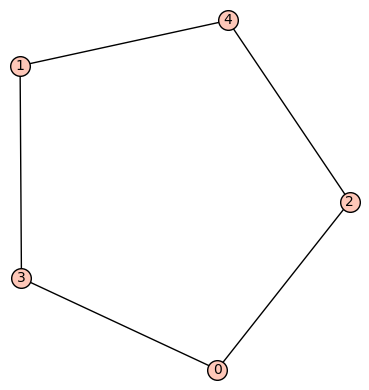
\includegraphics[width=5cm]{min_graf_5.2}
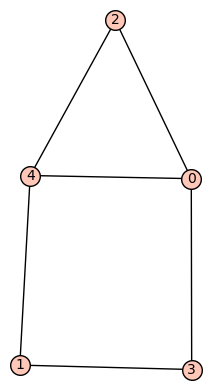
\includegraphics[width=5cm]{min_graf_5.3}
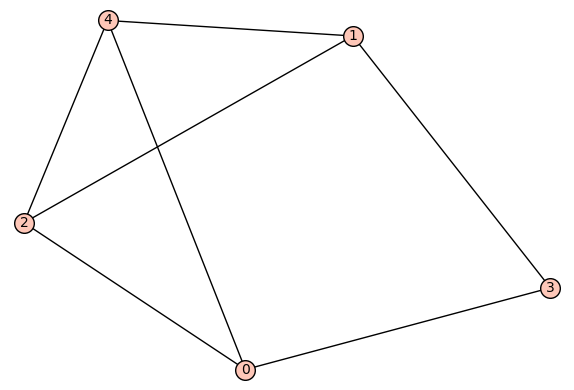
\includegraphics[width=5cm]{min_graf_5.4}
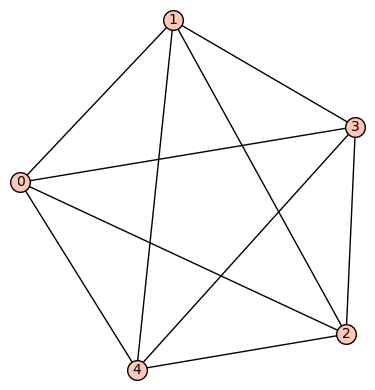
\includegraphics[width=5cm]{min_graf_5.5}

Pri grafih na šest vozliščih je razlika ponovno $0$. Od skupno $112$ vseh možnih grafov na šest vozliščih ima razliko $0$ natanko $28$ grafov. Program testira vse šestvozliščne grafe v približno $0.3$ sekunde. Spodaj je prikazanih par primerov.

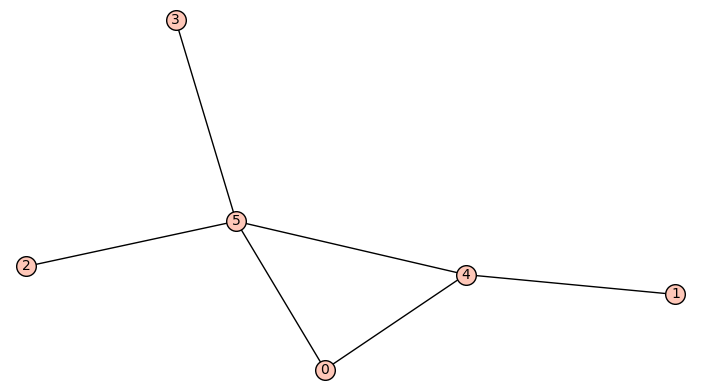
\includegraphics[width=5cm]{min_graf_6.1}
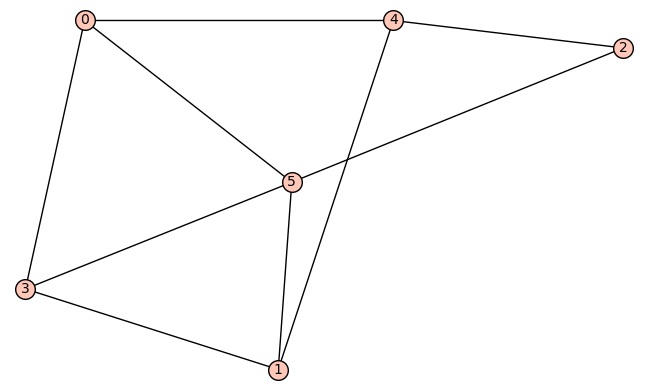
\includegraphics[width=5cm]{min_graf_6.2}
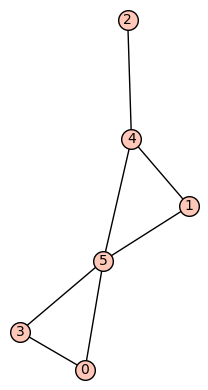
\includegraphics[width=5cm]{min_graf_6.3}
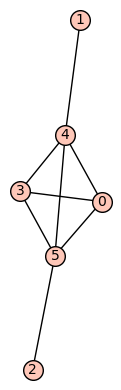
\includegraphics[width=5cm]{min_graf_6.4}
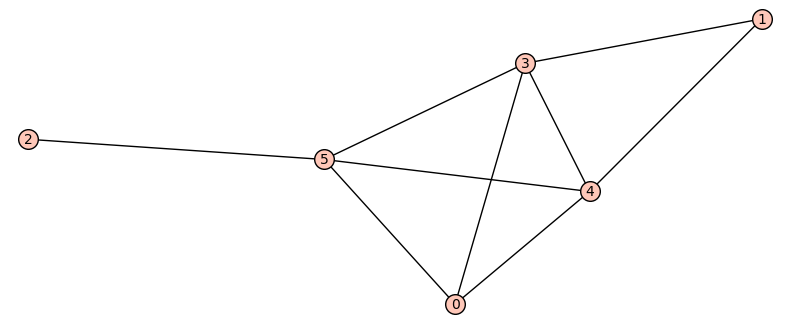
\includegraphics[width=5cm]{min_graf_6.5}

Za grafe na sedem vozliščih je minimalna razlika predpostavke ponovno $0$. Sedaj je možno generirati $853$ različnih grafov, razliko $0$ pa jih ima $223$. Program testira to predpostavko na vseh generiranih grafih na sedmih vozliščih v približno $2.5$ sekunde. Ponovno si poglejmo nekaj primerov teh grafov.

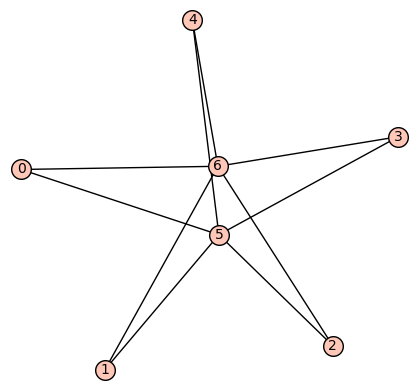
\includegraphics[width=5cm]{min_graf_7.1}
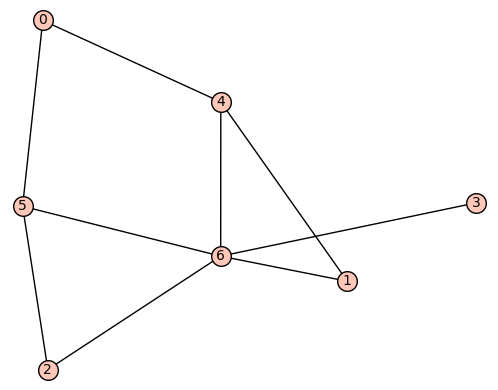
\includegraphics[width=5cm]{min_graf_7.2}
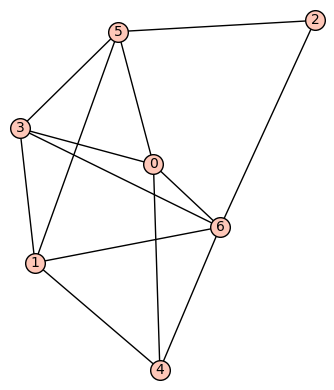
\includegraphics[width=5cm]{min_graf_7.3}
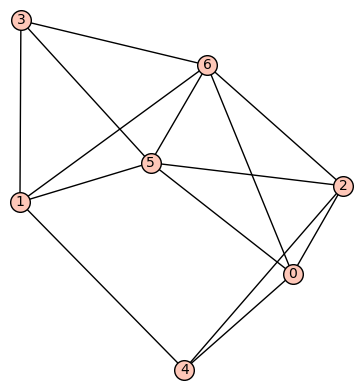
\includegraphics[width=5cm]{min_graf_7.4}
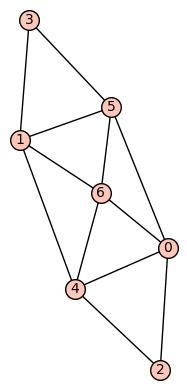
\includegraphics[width=5cm]{min_graf_7.5}

Grafi na osmih vozliščih imajo razliko leve in desne strani ponovno enako $0$. Zdaj generiramo že $11117$ različnih grafov in za njihovo testiranje porabimo že kar približno $55$ sekund. Grafov z osmimi vozlišči, kjer je razlika predpostavke enaka $0$ je $3374$.

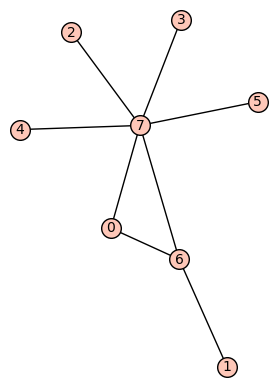
\includegraphics[width=5cm]{min_graf_8.1}
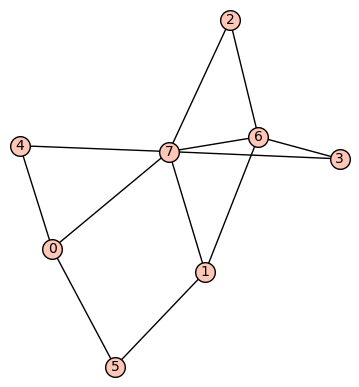
\includegraphics[width=5cm]{min_graf_8.2}
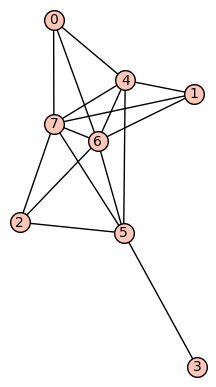
\includegraphics[width=5cm]{min_graf_8.3}
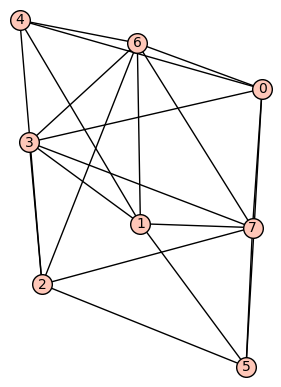
\includegraphics[width=5cm]{min_graf_8.4}
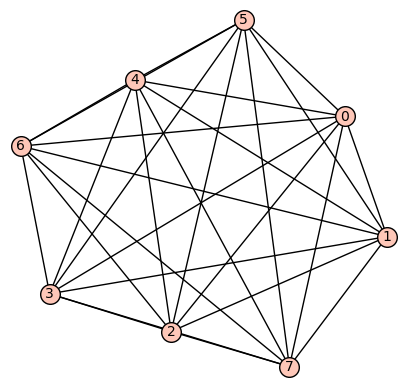
\includegraphics[width=5cm]{min_graf_8.5}

Za grafe na devetih vozliščih se konča naše preizkušanje majhnih grafov, ker na tej točki računalnik ni več sposoben generirati vseh preprostih povezanih grafov na devetih vozliščih preko generatorja  $graphs.nauty\_geng('v\ -c')$. Portal $CoCalc$ sam terminira generator, če je ta zagnan.

Iz vseh preverjenih majhnih grafov na do osem vozlišč pa lahko opazimo več stvari. Kot prvič, je bila minimalna razlika v predpostavki ne glede na število vozlišč enaka $0$. Tudi z izjemo grafa na dveh vozliščih, je bila razlika predpostavke enaka $0$, ko je imelo vsako vozlišče najmanj $2$ povezavi. Opazimo pa lahko še, da je bil med grafi, kjer je bila razlika predpostavke enaka $0$ vedno graf, kjer so bila vsa vozlišča povezana med seboj.

\end{document}